
\documentclass{article}

\usepackage{geometry}
\usepackage{amsmath}
\usepackage{soul}
\usepackage{color}
\usepackage{amssymb}
\usepackage{graphicx}
\usepackage{float}
\usepackage{cancel}
\usepackage{setspace}
\usepackage{listings}

%\definecolor{lightgrey}{rgba}{.824, .825, .825}
\definecolor{lightgrey}{rgb}{.867, .894, .886}

% no indentation
\setlength{\parindent}{0cm}

\lstdefinestyle{code}{
    backgroundcolor=\color{lightgrey},
    breaklines=true,
    numbers=left,
	basicstyle=\small,
    tabsize=4,
    language=Python
}
\lstset{style=code}

\newcommand{\mathsym}[1]{{}}
\newcommand{\unicode}[1]{{}}
\newcommand{\pd}[2]{\frac{\partial #1}{\partial #2}}

\newcommand{\eig}{\text{eig}}
\newcommand{\abs}{\text{abs}}

\geometry{a4paper, left=2cm, right=2cm, top=1cm, bottom=2cm}

\title{}
\author{Brooks Karlik}
\date{\today}

\newcommand{\rank}{\text{rank}}
\setlength{\parindent}{0.0pt}


\begin{document}

\maketitle
\newpage


$$
	F^*
	= 
	F^* 
	- 
	\alpha h^2 \rho
	\text{ }
	\abs
	\left(
		%du/du
		\pd{u}{x}
	\right)
	\pd{u}{x}
	\begin{bmatrix}
		0 \\
		1 \\
		u
	\end{bmatrix}
$$


Take the following code for LF method with two identical methods of solving for $q$: one with slicing, and one with raw indexing.
The output for the following code is in \ref{top}.

\begin{figure}[H]
	\centering
	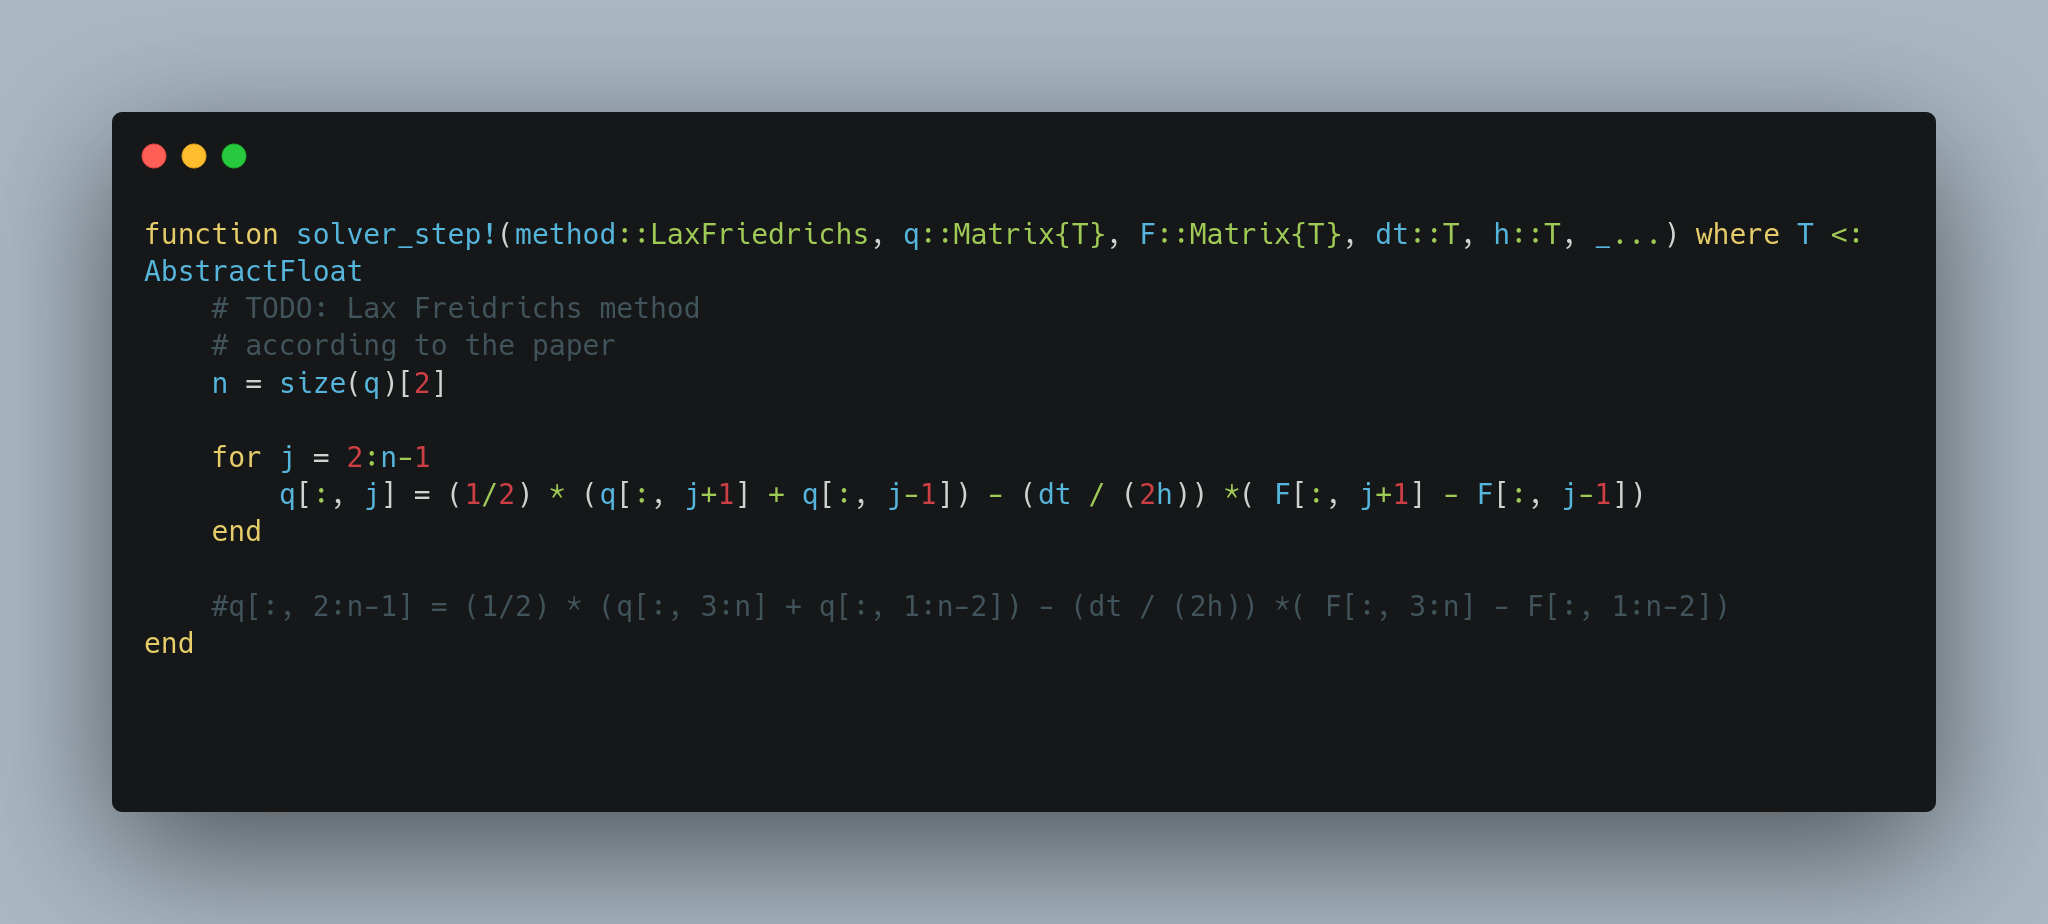
\includegraphics[width=\textwidth]{./figs/top.png}
\end{figure}

\begin{figure}[H]
	\centering
	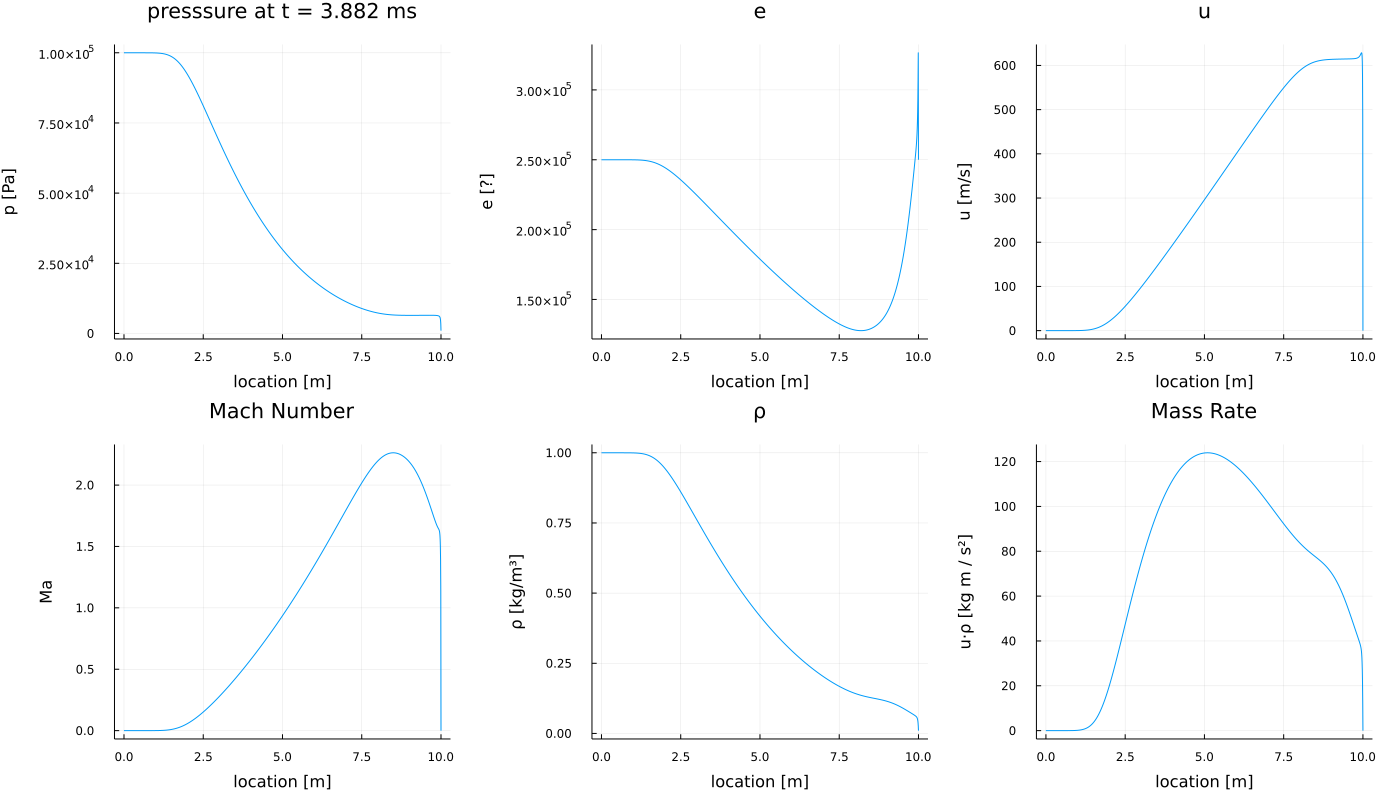
\includegraphics[width=\textwidth]{./figs/top_statement.png}
	\label{top}
	\caption{top statement only results}
\end{figure}

If we comment out the top statement and only run the bottom statement the results are in figure \ref{bottom}

\begin{figure}[H]
	\centering
	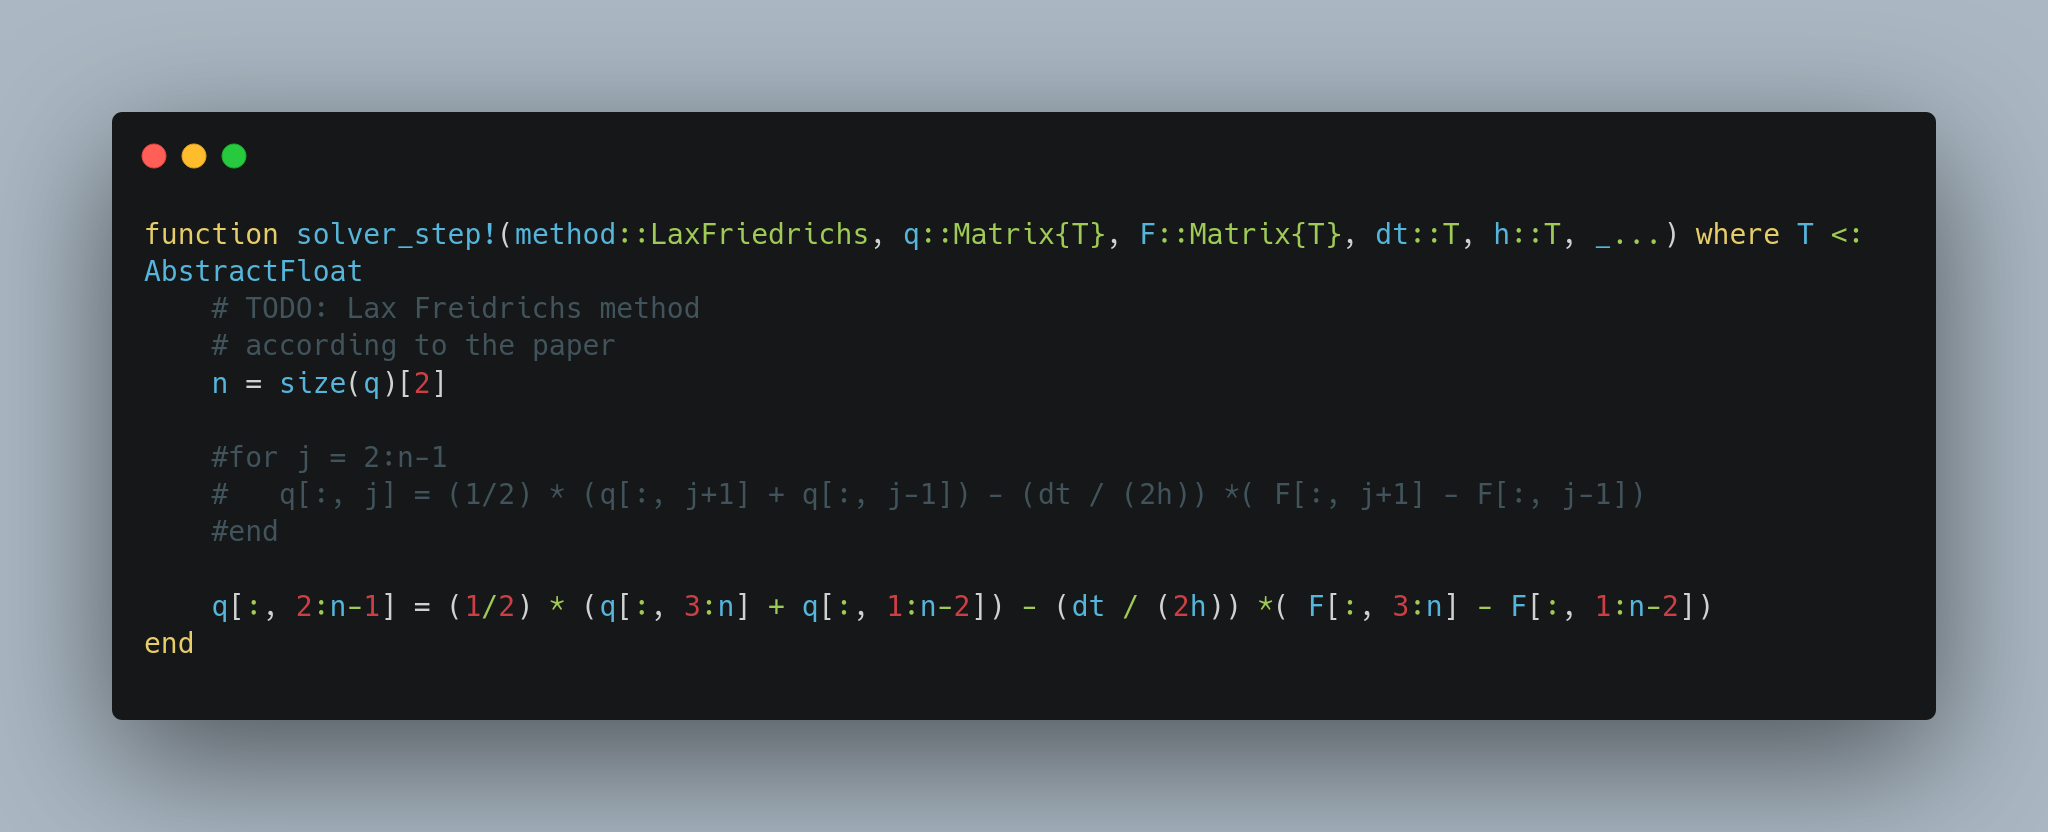
\includegraphics[width=\textwidth]{./figs/bottom.png}
\end{figure}

\begin{figure}[H]
	\centering
	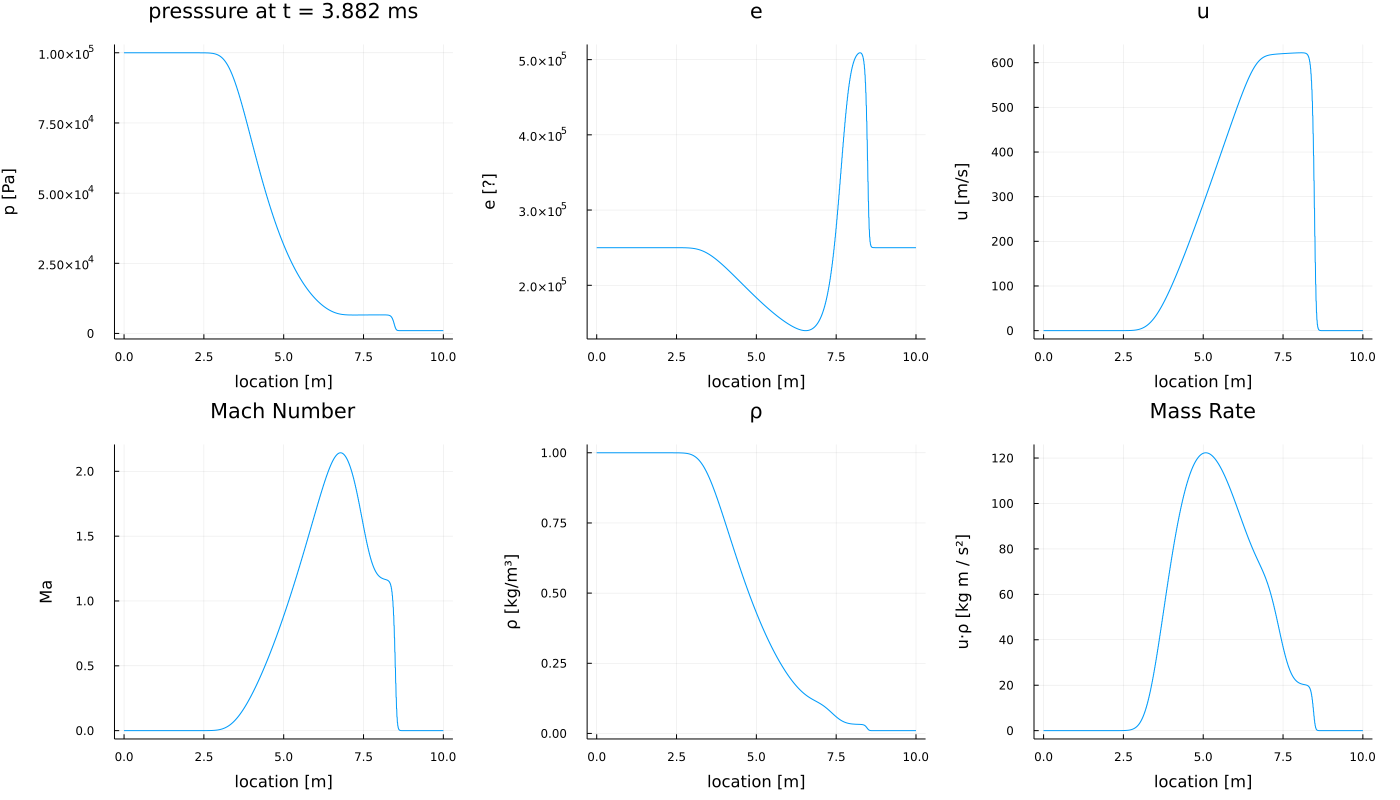
\includegraphics[width=\textwidth]{./figs/bottom_statement.png}
	\caption{bottom statement only results}
	\label{bottom}
\end{figure}

If we run both statements, the result is in figure \ref{both}.

\begin{figure}[H]
	\centering
	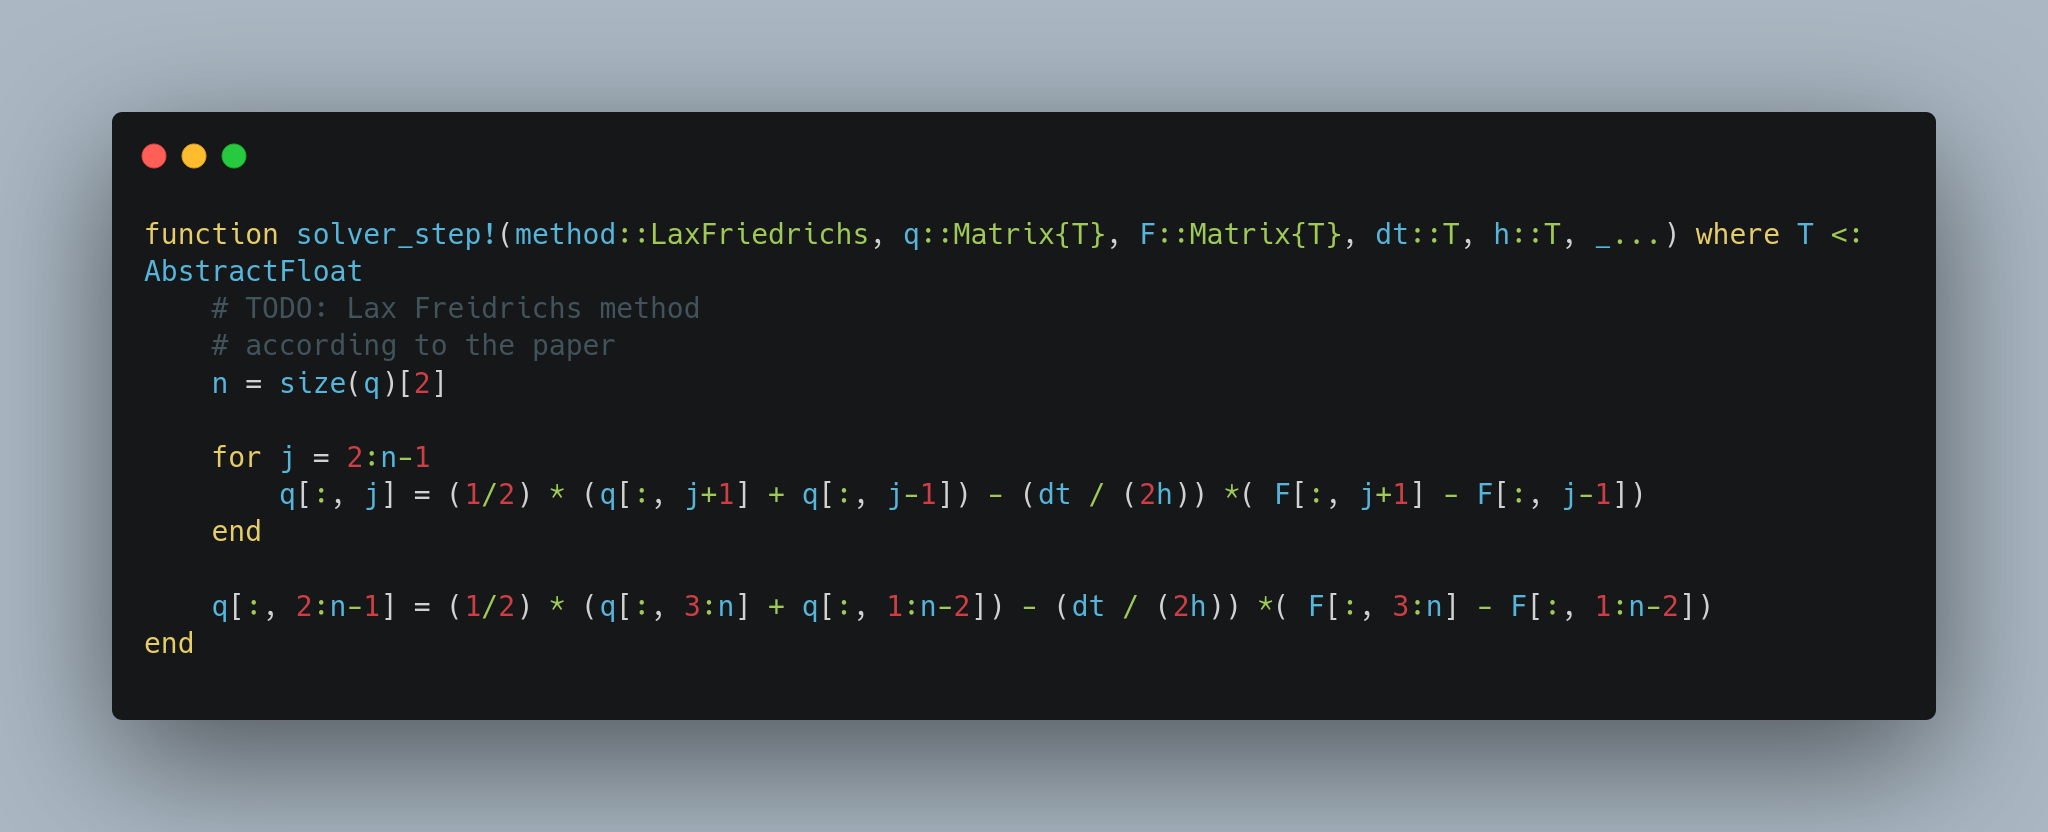
\includegraphics[width=\textwidth]{./figs/both.png}
\end{figure}

\begin{figure}[H]
	\centering
	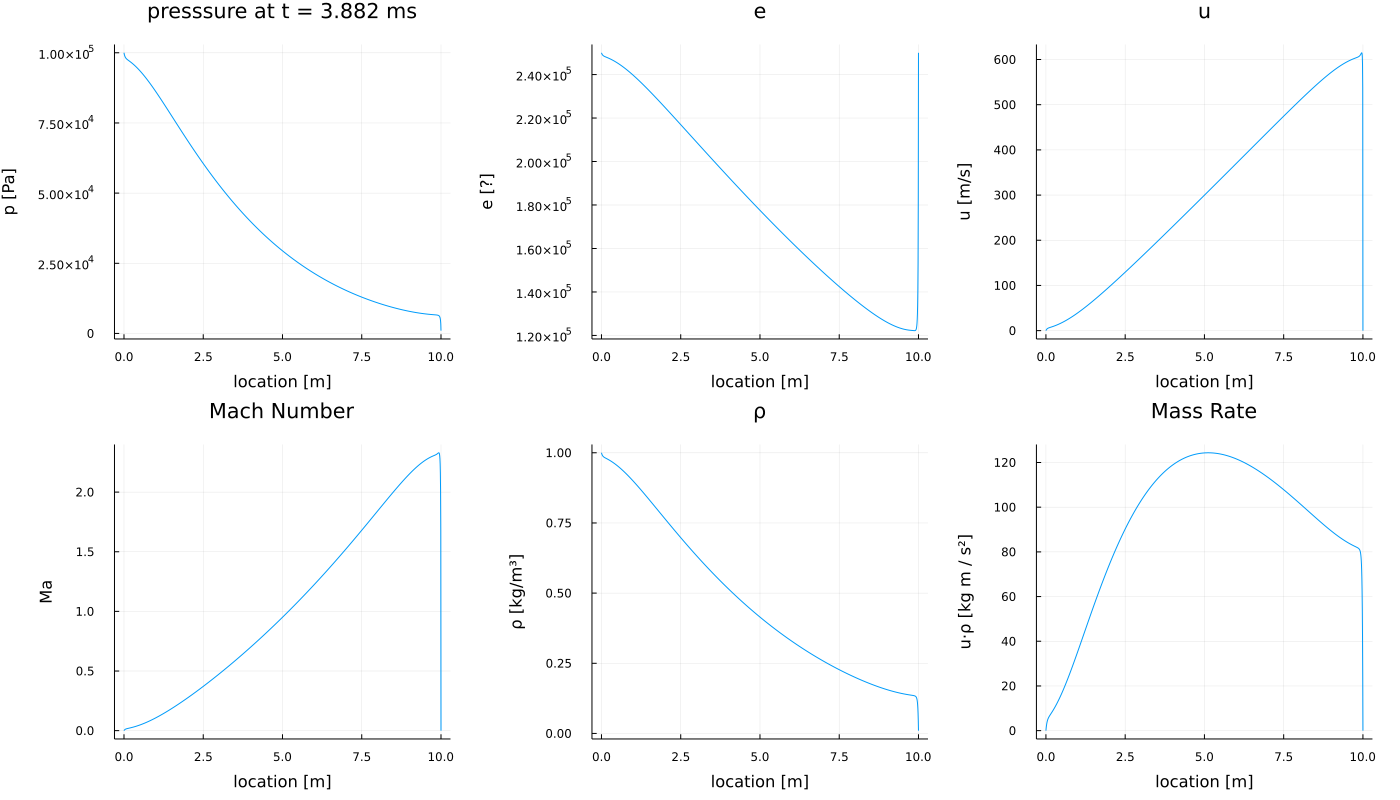
\includegraphics[width=\textwidth]{./figs/both_statements.png}
	\caption{both statements results}
	\label{both}
\end{figure}

\end{document}
